% Source: Code/xband-radar-sim/docs/radar_simulation_technical.tex
% Description: Objects represented as triangle meshes. Left: Corner reflector (3 triangles). Right: Sphere approximated by icosphere subdivision.

\documentclass[border=4pt]{standalone}
\usepackage{algpseudocode}
\usepackage{amsmath,amssymb,amsfonts}
\usepackage[T1]{fontenc}
\usepackage{graphicx}
\usepackage{pgfplots}
\usepackage{tikz}
\usepackage{xcolor}
\pgfplotsset{compat=1.18}
\usetikzlibrary{arrows.meta,positioning,shapes.geometric,calc,patterns,decorations.pathmorphing,3d,angles,quotes}

\definecolor{radargreen}{RGB}{0,255,0}
\definecolor{raycolor}{RGB}{255,165,0}
\definecolor{targetcolor}{RGB}{255,0,0}
\definecolor{groundcolor}{RGB}{139,90,43}
\definecolor{skycolor}{RGB}{135,206,235}
\definecolor{beamcolor}{RGB}{255,255,0}


\begin{document}
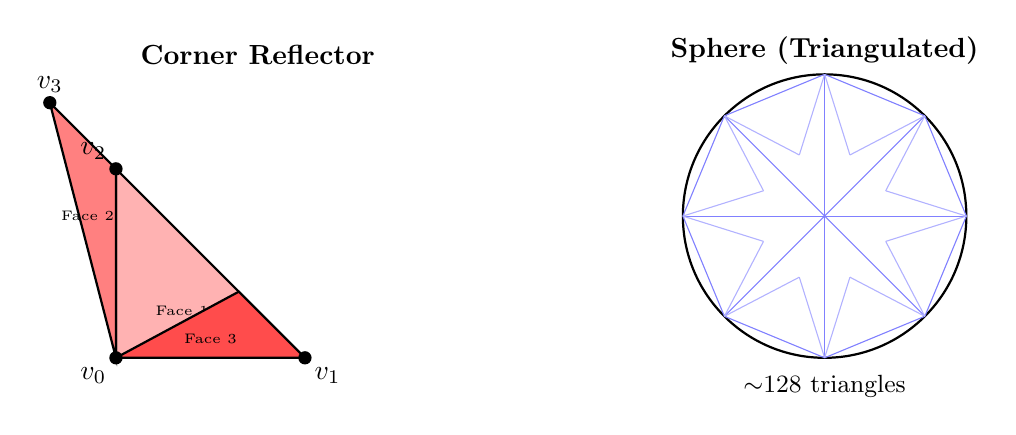
\begin{tikzpicture}[scale=1.2]
    % Corner reflector triangles
    \begin{scope}[shift={(0,0)}]
        \node[above] at (1.5,3) {\textbf{Corner Reflector}};

        % XY plane
        \fill[red!30] (0,0) -- (2,0) -- (0,2) -- cycle;
        \draw[thick] (0,0) -- (2,0) -- (0,2) -- cycle;
        \node at (0.7,0.5) {\tiny Face 1};

        % YZ plane (projected)
        \fill[red!50] (0,0) -- (0,2) -- (-0.7,2.7) -- cycle;
        \draw[thick] (0,0) -- (0,2) -- (-0.7,2.7) -- cycle;
        \node at (-0.3,1.5) {\tiny Face 2};

        % XZ plane (projected)
        \fill[red!70] (0,0) -- (2,0) -- (1.3,0.7) -- cycle;
        \draw[thick] (0,0) -- (2,0) -- (1.3,0.7) -- cycle;
        \node at (1,0.2) {\tiny Face 3};

        % Vertex labels
        \fill (0,0) circle (2pt) node[below left] {$v_0$};
        \fill (2,0) circle (2pt) node[below right] {$v_1$};
        \fill (0,2) circle (2pt) node[above left] {$v_2$};
        \fill (-0.7,2.7) circle (2pt) node[above] {$v_3$};
    \end{scope}

    % Sphere approximation
    \begin{scope}[shift={(6,0)}]
        \node[above] at (1.5,3) {\textbf{Sphere (Triangulated)}};

        % Draw icosphere-like mesh
        \draw[thick] (1.5,1.5) circle (1.5);

        % Triangle subdivisions
        \foreach \a in {0,45,...,315} {
            \draw[thin, blue!50] (1.5,1.5) -- ({1.5+1.5*cos(\a)},{1.5+1.5*sin(\a)});
        }
        \foreach \a in {0,45,...,315} {
            \draw[thin, blue!50] ({1.5+1.5*cos(\a)},{1.5+1.5*sin(\a)}) -- ({1.5+1.5*cos(\a+45)},{1.5+1.5*sin(\a+45)});
        }

        % Inner ring
        \foreach \a in {22.5,67.5,...,337.5} {
            \draw[thin, blue!30] ({1.5+0.7*cos(\a)},{1.5+0.7*sin(\a)}) -- ({1.5+1.5*cos(\a-22.5)},{1.5+1.5*sin(\a-22.5)});
            \draw[thin, blue!30] ({1.5+0.7*cos(\a)},{1.5+0.7*sin(\a)}) -- ({1.5+1.5*cos(\a+22.5)},{1.5+1.5*sin(\a+22.5)});
        }

        \node at (1.5,-0.3) {\small $\sim$128 triangles};
    \end{scope}
\end{tikzpicture}
\end{document}
